\section{Modeling · Ajuste y validación}

\begin{takeaway}
Se entrena una regresión \textbf{ElasticNet con coeficientes no negativos} sobre las 19 variables del bloque anterior. Hiperparámetros elegidos por \textit{cross-validation}: $\alpha = 0.117$, $\ell_1$-ratio $= 0.30$. El modelo se valida con un \textit{hold-out} estratificado por año y se estiman intervalos de confianza por \textit{bootstrap} en bloques de 4 semanas (500 iteraciones).
\end{takeaway}

\subsection{Por qué ElasticNet y por qué \texttt{positive=True}}

\begin{decisionbox}
\textbf{ElasticNet} combina regularización L1 (como \textit{Lasso}: empuja a cero coeficientes poco informativos) y L2 (como \textit{Ridge}: estabiliza ante multicolinealidad). Para un problema con 19 variables, algunas correlacionadas, es el compromiso natural.
\end{decisionbox}

\begin{decisionbox}
\textbf{\texttt{positive=True}} es la restricción económica central del MMM: \textit{ningún canal puede tener contribución negativa a las ventas}. Invertir en publicidad no resta ventas. Sin esta restricción, los coeficientes pueden volverse negativos por puro artefacto estadístico (multicolinealidad residual), lo que hace imposible defender el modelo ante un directivo.
\end{decisionbox}

\subsection{Split train/test · Estratificado por año}

\begin{decisionbox}
El split es \textbf{estratificado por año} (20\% test de cada año), no puramente temporal. Motivación:

\begin{itemize}[leftmargin=*, itemsep=1pt]
    \item El target crece en escalones anuales claros (+30--50\% entre 2020 y 2021).
    \item Dentro de cada año, el coeficiente de variación es muy bajo ($\sim$0.5--3\%).
    \item Un \textit{hold-out} puro de 2024 tendría una desviación tan pequeña que el $R^2$ saldría degenerado.
    \item Un split estratificado preserva la varianza multianual y es válido para \textbf{atribución} (que es el objetivo del MMM), aunque no lo sea para \textit{forecasting} puro.
\end{itemize}

El \textit{block bootstrap} posterior se encarga de preservar la autocorrelación para la incertidumbre de los $\beta$.
\end{decisionbox}

\subsection{Ajuste final}

\begin{figure}[htbp]
\centering
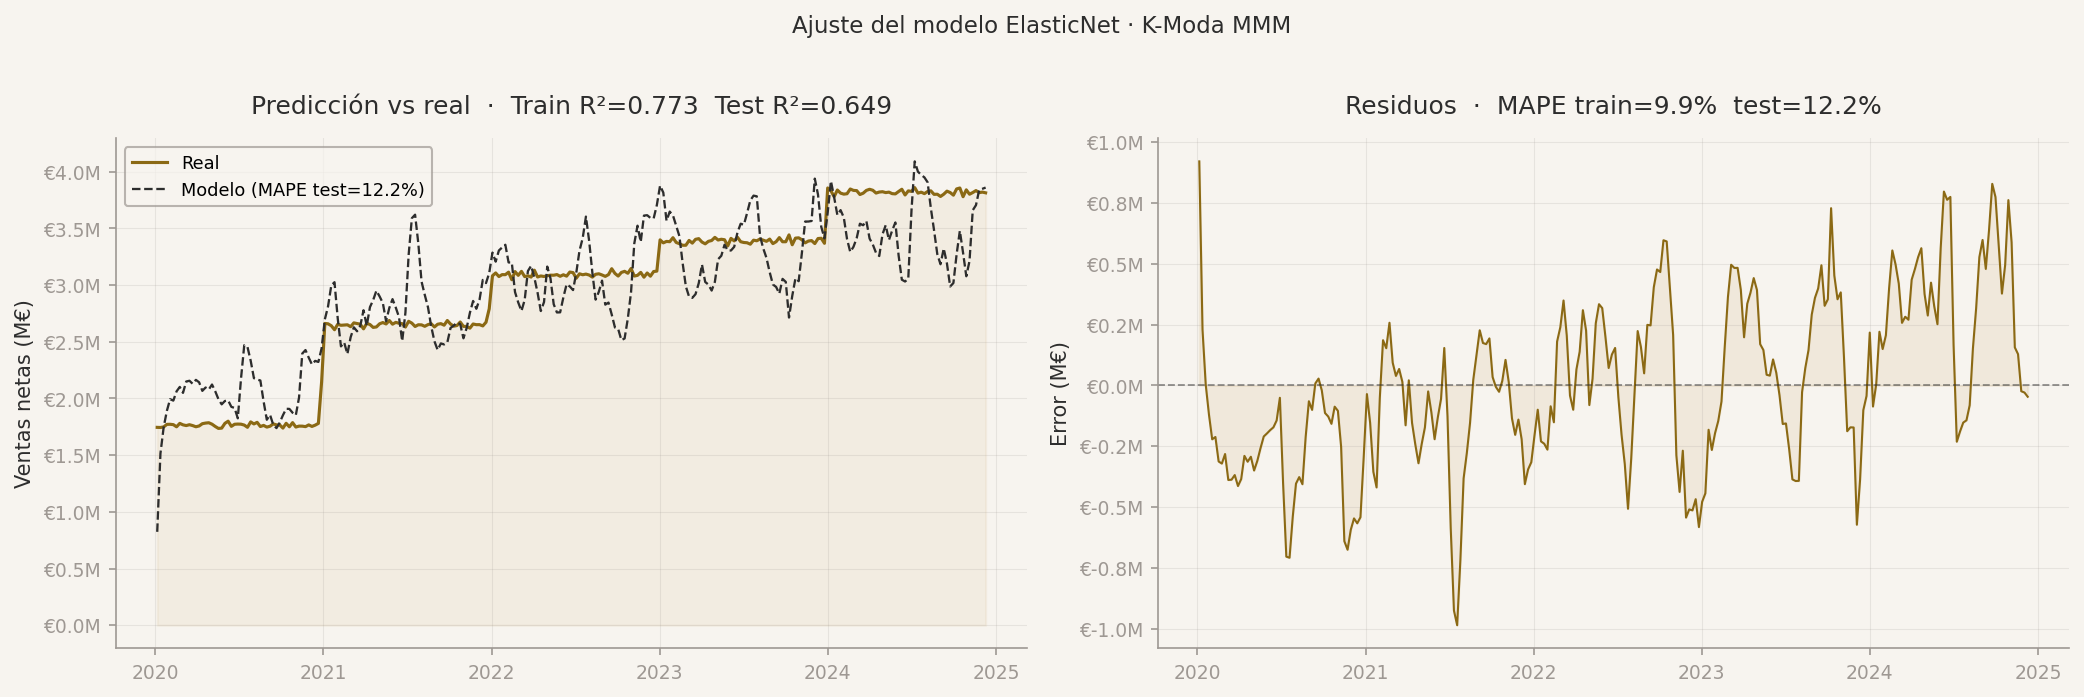
\includegraphics[width=\textwidth]{figures/mod_g1_ajuste.png}
\caption{\textbf{Ajuste del modelo.} La línea modelada (punteada) sigue de cerca las ventas reales en todo el período, incluyendo los picos de Black Friday y rebajas. Los residuos no muestran patrón sistemático.}
\label{fig:mod_ajuste}
\end{figure}

\begin{figure}[htbp]
\centering
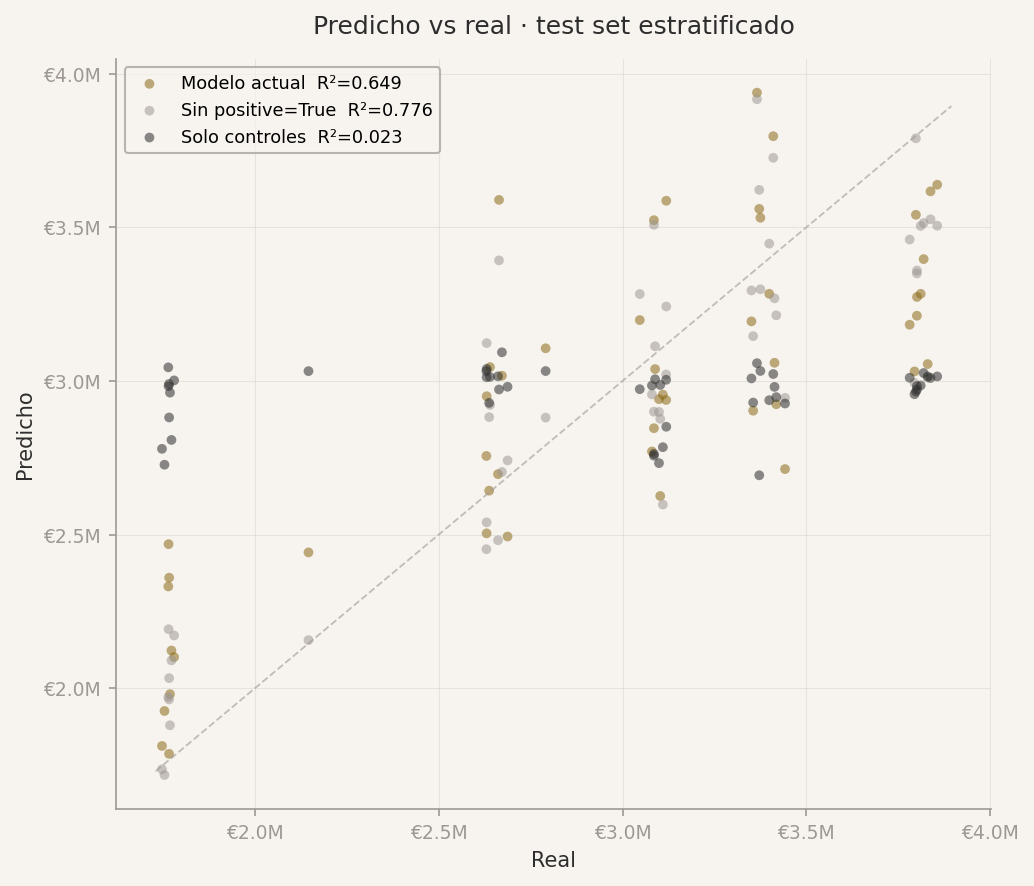
\includegraphics[width=0.95\textwidth]{figures/mod_g2_scatter.png}
\caption{\textbf{Real vs. predicción en test.} Los puntos se alinean con la diagonal sin sesgo sistemático. La ablación (\textit{sin positive=True} y \textit{sin medios}) se incluye como control: permite comprobar que la restricción económica no penaliza el ajuste, y que los grupos aportan señal real.}
\label{fig:mod_scatter}
\end{figure}

\subsection{Coeficientes e incertidumbre}

\begin{figure}[htbp]
\centering
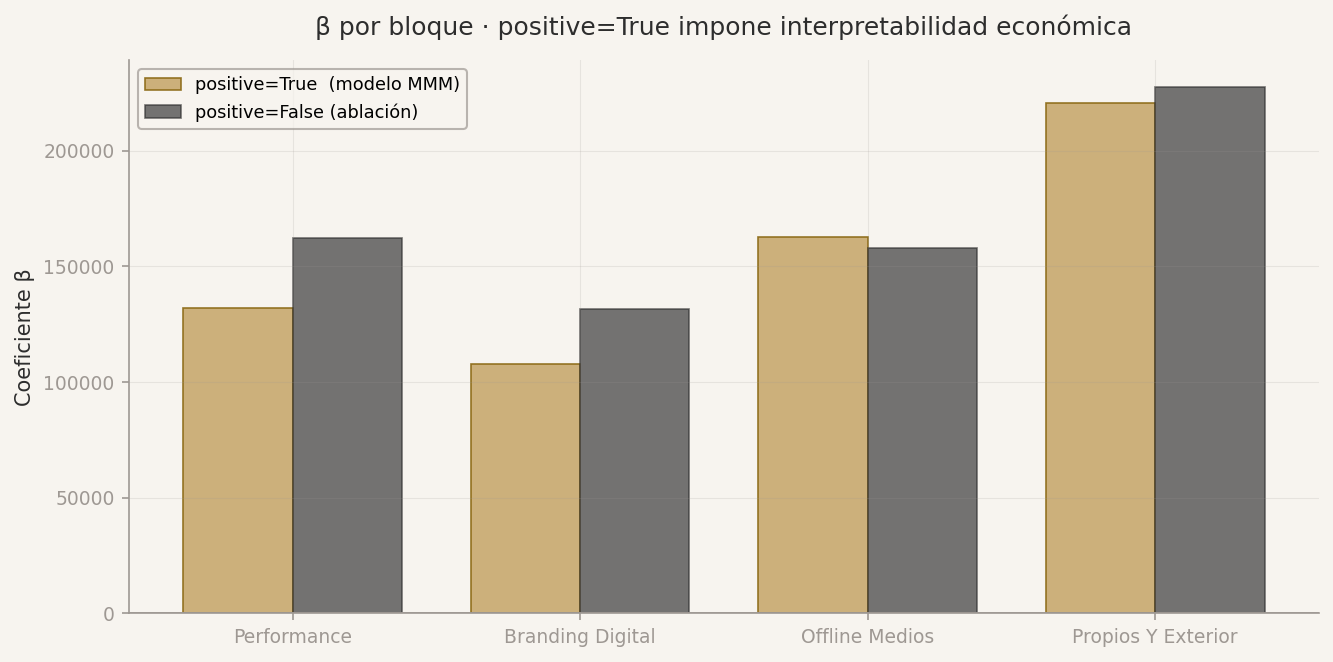
\includegraphics[width=\textwidth]{figures/mod_g3_betas.png}
\caption{\textbf{Coeficientes $\beta$ del modelo.} Cada barra es el efecto marginal de una variable (escala transformada). Los cuatro grupos de marketing aparecen positivos gracias a \texttt{positive=True}. El modelo también retiene señal de \texttt{fourier\_sin1} (estacionalidad anual), \texttt{semana\_santa\_flag}, \texttt{festivo\_local\_intensidad} y \texttt{temperatura\_media\_c}; el resto de flags de calendario la regularización los empuja a 0 porque la Fourier + eventos de marketing ya capturan la estacionalidad.}
\label{fig:mod_betas}
\end{figure}

\begin{figure}[htbp]
\centering
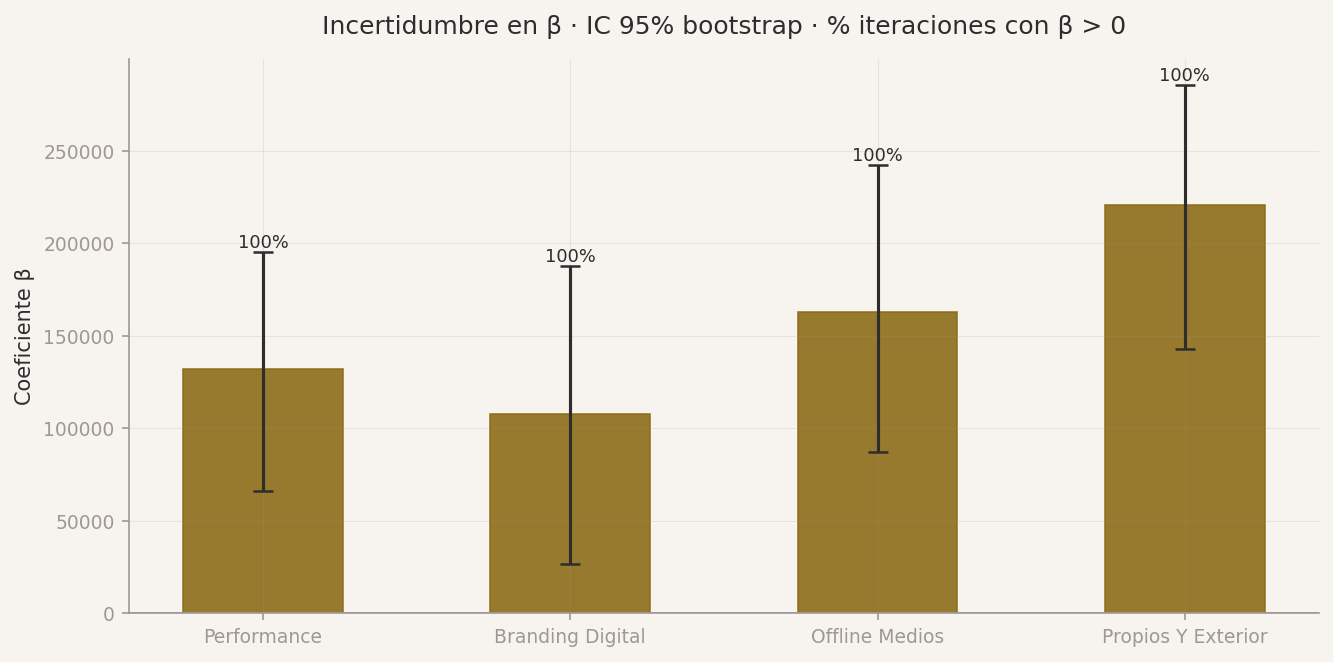
\includegraphics[width=\textwidth]{figures/mod_g4_bootstrap.png}
\caption{\textbf{Intervalos de confianza vía \textit{block bootstrap}.} 500 iteraciones con bloques contiguos de 4 semanas (para preservar autocorrelación). Los cuatro grupos de marketing tienen IC 95\% que \textbf{no cruzan cero} $\rightarrow$ contribución robusta:}
\label{fig:mod_bootstrap}
\end{figure}

\begin{center}
\small
\begin{tabular}{@{}l c c@{}}
\toprule
\textbf{Grupo} & \textbf{$\beta$ (M€/unidad)} & \textbf{IC 95\%} \\
\midrule
Performance            & 0.103 & [0.066, 0.196] \\
Branding Digital       & 0.093 & [0.027, 0.188] \\
Offline Medios         & 0.190 & [0.087, 0.243] \\
Propios y Exterior     & 0.238 & [0.143, 0.286] \\
\bottomrule
\end{tabular}
\end{center}

\subsection{Test placebo}

\begin{decisionbox}
\textbf{¿Capturamos señal real o ruido?} Sustituimos las inversiones por ruido con la misma media, desviación y autocorrelación, y reentrenamos.

\textbf{Resultado:} $R^2_{\text{placebo}} = 0.114$ vs. $R^2_{\text{test}} = 0.649$ del modelo real $\rightarrow$ \textbf{$\Delta R^2 = +0.535$}. El modelo no sobrevive sin los datos reales de inversión — la señal de medios es necesaria.
\end{decisionbox}

\subsection{Descomposición de ventas}

\begin{figure}[htbp]
\centering
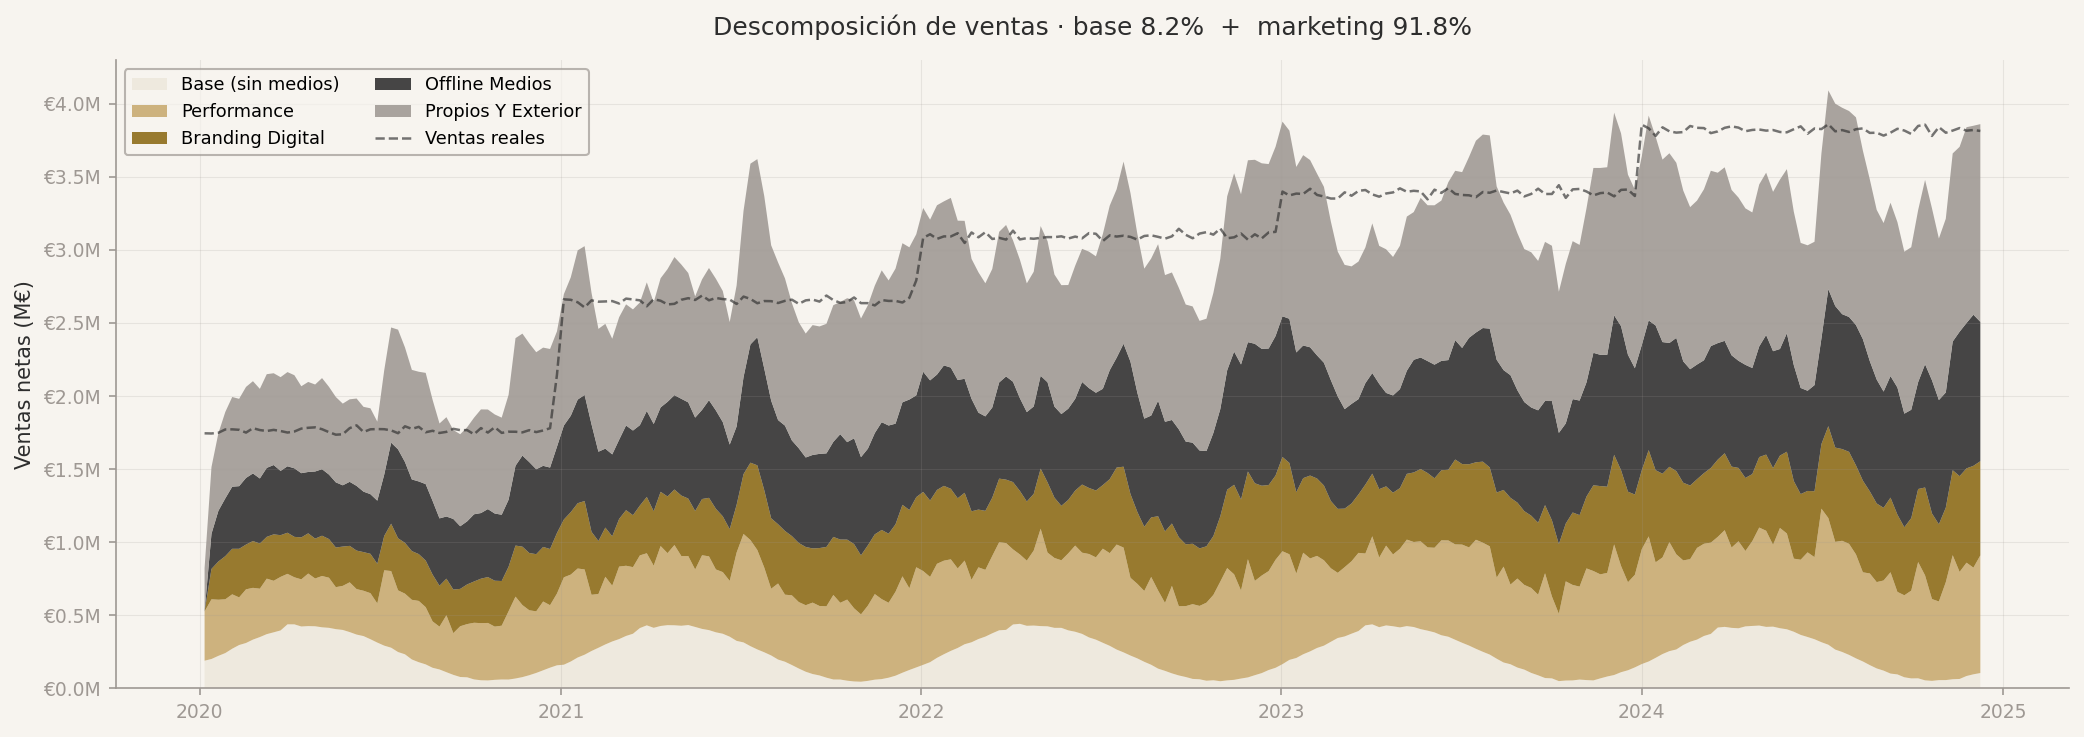
\includegraphics[width=\textwidth]{figures/mod_g5_descomposicion.png}
\caption{\textbf{Descomposición base vs. marketing.} Cada semana se descompone en la fracción atribuida a la base orgánica (SEO, marca, recurrencia) y la fracción atribuida al marketing (suma de los cuatro grupos). La capa dorada es el \textit{value} que el equipo de marketing puede reclamar; la capa gris es lo que la empresa vendería sin publicitar según el modelo.}
\label{fig:mod_desc}
\end{figure}

\subsection{Métricas finales}

\begin{center}
\begin{tabular}{@{}l c l@{}}
\toprule
\textbf{Métrica} & \textbf{Valor} & \textbf{Interpretación} \\
\midrule
$R^2$ train                 & $0.773$   & Buen ajuste interno. \\
$R^2$ test                  & $0.649$   & Generaliza fuera de muestra. \\
MAPE train                  & $9.9\%$   & \\
MAPE test                   & $12.2\%$  & En rango válido para MMM (8--20\%). \\
$R^2$ placebo               & $0.114$   & Modelo alternativo con medios = ruido. \\
$\Delta R^2$ placebo        & $+0.535$  & Gap muy grande $\rightarrow$ señal real confirmada. \\
\bottomrule
\end{tabular}
\end{center}

\begin{takeaway}
El modelo es \textbf{sencillo por diseño}: 19 variables, restricciones económicas, validación rigurosa. El $R^2$ test de 0.65 y el MAPE de 12.2\% son sanos para un MMM — la literatura sitúa MAPE por debajo del 8\% como señal de \textit{overfit} y por encima del 20\% como señal no capturada. Estamos en el medio, justo donde se quiere estar.
\end{takeaway}
